\documentclass[../main.tex]{subfiles}

\begin{document}

RDF es un lenguaje de modelado para describir recursos en la web. RDF permite modelar recursos (datos) y sus relaciones mediante un grafo dirigido.

\hfill

Se ha tenido que desarrollar un mapa de clases que están relacionados mediante propiedades de datos. Definiendo las clases, operaciones:

\hfill

\begin{figure}[ht]
    \centering
    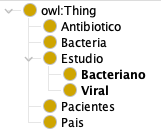
\includegraphics[scale=0.65]{images/clasesport.png}
    \caption{Clases}
    \label{clasesport}
\end{figure}


\begin{figure}[h]
    \centering
    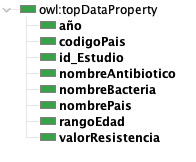
\includegraphics[scale=0.65]{images/porpieddes .png}
    \caption{Relaciones}
    \label{Relaciones}
\end{figure}

El mapa se ha jerarquizado en torno al estudio que se esta realizando, de el parten las relaciones.

\newpage

Para expresar atributos de las clases se han creado propiedades:

\hfill

\begin{figure}[ht]
    \centering
    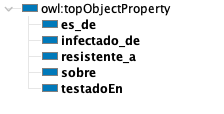
\includegraphics[scale=0.65]{images/operaciones.png}
    \caption{Clases}
    \label{operaciones}
\end{figure}

Estas propiedades complementan a ciertas clases, aportando información sobre ellas. La mayoría se trata de propiedades de una clase a un tipo de dato int o string peor rango de edad se ha declarado como un enumerado.

\hfill

\begin{figure}[ht]
    \centering
    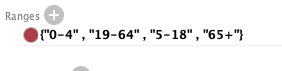
\includegraphics[scale=0.65]{images/reeee.png}
    \caption{}
    \label{reeee}
\end{figure}
\end{document}